\chapter{openPOWERLINK}
\label{cha:oplk}
openPOWERLINK is an Open Source implementation of the POWERLINK protocol.
The implementation contains the openPOWERLINK stack and different demo applications for various platforms.
It is designed for an simple introduction into POWERLINK and an public available implementation.
This project should allow manufacturers an easily integration of POWERLINK into their projects.
The Open Source implementation targets an improved integration and development of new features which may be inspired by request of manufacturers and other users.
The stack is distributed under the \emph{BSD} license and is available at Github \cite{openpowerlink_github} and Sourceforge \cite{openpowerlink_sourceforge}.

This following chapter will discuss the properties, structure and functionalities of POWERLINK.

\section{POWERLINK}
\label{sec:oplk_powerlink}
POWERLINK is an industrial real-time communication protocol based on the IEEE 802.3 standard (Fast Ethernet \cite{ethernet_ieee_2016}).
POWERLINK was developed by the members of the Ethernet POWERLINK Standardization Group (\emph{EPSG}).
The \emph{EPSG} consists of different companies located in the fields of real time communications, automation and field bus communication. \cite{epsg_hp}

One fundamental principle of POWERLINK is the usage of a common communication system for various applications.
I.e POWERLINK supports the real-time transmission of data for time critical applications and a simultaneous transmission of less time critical asynchronous information.

For granting a deterministic communication, which is essential for real-time communication, collisions within a POWERLINK network are prevented by the definition of the POWERLINK cycle.
Therefore the features of collision detection and transmission retires of Ethernet Carrier Sense Multiple Access/Collision Detection (\emph{CSMA/CD}) are not necessary for a POWERLINK network. \cite[section 4.2]{ethernet_ieee_2016}
This collision prevention is done via strict slot based transmission.
Each node within a POWERLINK network is only allowed to send within its assigned slot and furthermore each controlled node (\emph{CN}) is only permitted to send as response to the managing node (\emph{MN}). \cite[chapter 1]{epsg_epsg_2013}
The communication sequence of a standard POWERLINK network is shown in section \ref{sec:oplk_powerlink_commcycle}.

The structure and components of a POWERLINK network are described in the following section.

\subsection{Network structure}
\label{sec:oplk_powerlink_network}
A POWERLINK network consists of the following two different node types.

\begin{description}
    \item[MN] The managing node exist once within a normal POWERLINK network and controls the communication flow.
    The MN manages all registered network participants, provides a clock and defines the transmission cycle.
    \item[CN] All other nodes within a normal POWERLINK network are controlled nodes and react according to the controls of the \emph{MN}.
\end{description}

Within a POWERLINK network unique POWERLINK addresses (Node IDs) are assigned to each node.
The address range from 1 to 239 is available for all \emph{CNs} and can be assigned freely.
The address 240 is fixed for the \emph{MN}, each node assigned the Node ID 240 automatically performs as \emph{MN}.
When the execution of the \emph{MN} role is not possible the assignment of the Node ID 240 is not permitted.
\cite{epsg_epsg_2013}

A simple POWERLINK network consisting of a \emph{MN} connected to one \emph{CN} directly and additional two \emph{CNs} via a Ethernet HUB is shown in figure \ref{fig:powerlink_network}.

\begin{figure}
    \centering
    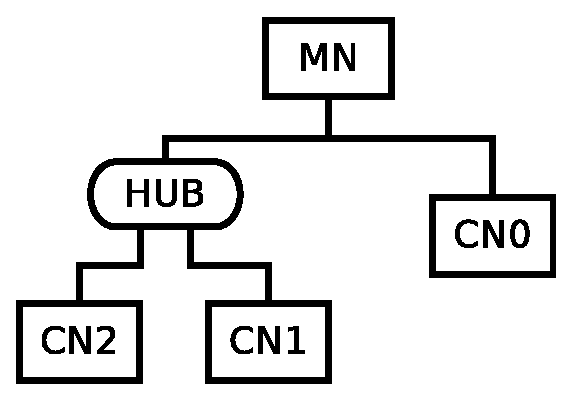
\includegraphics[width=0.5\linewidth]{powerlink_network}
    \caption{POWERLINK network consisting of a \emph{MN} connected to one \emph{CN} and a Ethernet HUB which is connected to two more \emph{CNs}.}
    \label{fig:powerlink_network}
\end{figure}

POWERLINK is based on the standard IEEE 802.3 MAC layer and therefore the usage of default Ethernet hardware is possible.
The different nodes can be arranged in various topologies.
Recommended is the integration of Ethernet HUBs into each node for allowing an easy setup of common used network structures, e.g. a star topology with lines of multiple nodes. \cite[chapter 3]{epsg_epsg_2013}

\subsection{Frame}
\label{sec:oplk_powerlink_frame}
The POWERLINK frame is embedded in the payload of an Ethernet 2 frame and is defined via the Ether type 0x88AB.
Therefore the POWERLINK frame is preceded by the Ethernet 2 Header containing destination \emph{MAC} Address, source \emph{MAC} Address and Ether type.
The payload of an Ethernet 2 Frame can reach up to a length of 1500 bytes succeeding with 4 bytes checksum. \cite[section 3.2]{ethernet_ieee_2016} \cite[section 4.6.1]{epsg_epsg_2013}

In figure \ref{fig:powerlink_frame} the structure of a POWERLINK frame is shown.
The POWERLINK header shown to the left contains the destination and source Node Id preceded by the message type.
The payloads length and content is depending on the transmitted message and thereby defined by the message type. \cite[section 4.6.1.1]{epsg_epsg_2013}

\begin{figure}
    \centering
    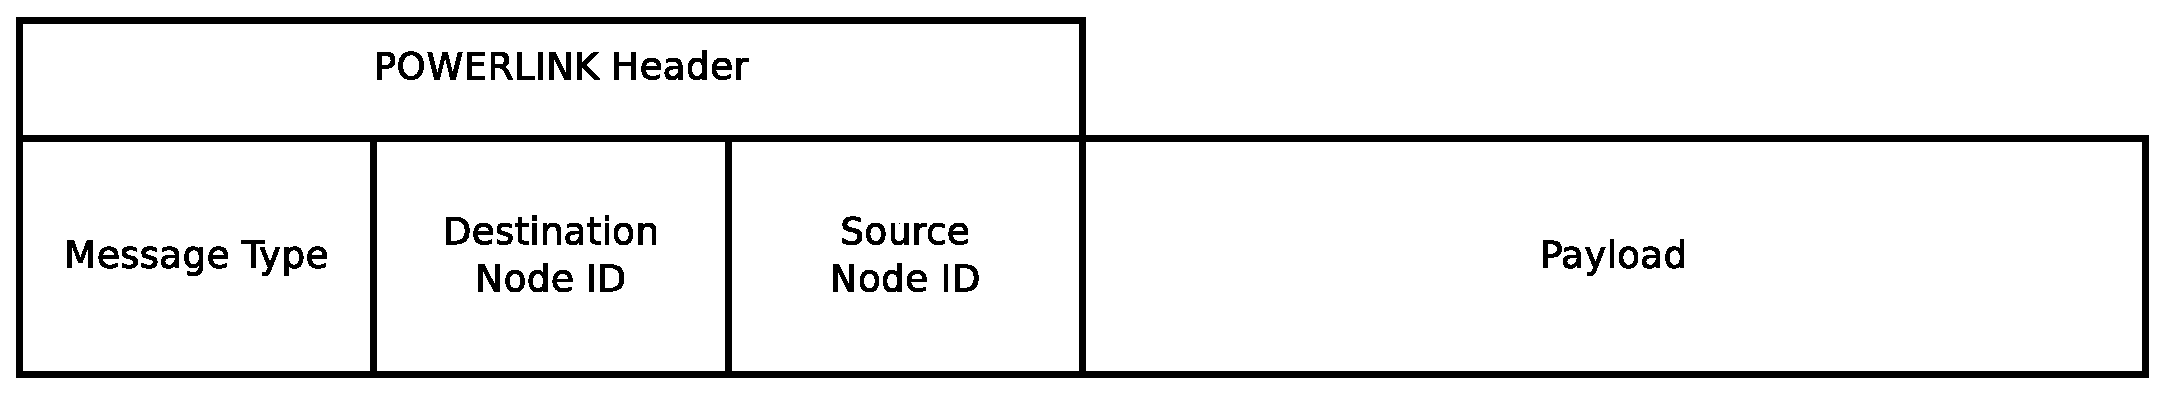
\includegraphics[width=0.9\linewidth]{powerlink_frame}
    \caption{POWERLINK frame showing POWERLINK header and payload.}
    \label{fig:powerlink_frame}
\end{figure}

Detailed information about the different structures of transmitted payloads depending on the message type can be found here \cite[section 4.6.1.1.1]{epsg_epsg_2013}

\subsection{Commands}
\label{sec:oplk_powerlink_commands}

As mentioned above different transmitted POWERLINK messages are defined via the message type.
The following commands are distinguished by the according message type.

\begin{description}
    \item[Soc] Start of cycle is sent by the \emph{MN} as multicast and defines the start of the POWERLINK cycle and the isochronous phase.
    \item[PReq] Poll request is sent by the \emph{MN} to a specific \emph{CN} transmitting data and requesting the transmission data from the \emph{CN}.
    \item[PRes] Poll response is sent by the \emph{CN} as multicast as response to a \emph{PReq} and contains data from the \emph{CN}.
    \item[SoA] Start of Asynchronous is sent by the \emph{MN} as multicast and defines the end of the isochronous phase and the begin of the asynchronous phase.
    Additionally the \emph{SoA} message contains the information about the assignment of the following asynchronous slot.
    \item[ASnd] Asynchronous send is sent either by the \emph{MN} or a \emph{CN} as multicast and contains asynchronous data.
\end{description}

The transmission of an \emph{ASnd} message is happening in the asynchronous phase, as described in the next section.
\emph{Asnd} messages can embody different services which are shown in the following listing.\cite[section 4.6.1.1.6.1]{epsg_epsg_2013}

\begin{description}
    \item[IdentResponse] represents a response to a received \emph{IdentRequest}.
    \item[StatusResponse] represents a response to a received \emph{StatusRequest}.
    \item[NMTRequest] represents a response to a received \emph{NMTRequestInvite} when a \emph{NMT} request is pending at the local node.
    \item[NMTCommand] represents a response to a received \emph{NMTRequestInvite} when a \emph{NMT} command is pending at the local node.
    \item[SDO] represents a response to a received \emph{UnspecifiedInvite} and signals an included \emph{SDO} transmission.
    \item[Manufacturer specific] represents manufacturer specific services and usages.
\end{description}

This transmissions are invoked by the preceding \emph{SoA}, which includes an request service id.
According to this request service id the scheduled node is responding with the according response.
The possible requested service ids are shown in the following listing. \cite[section 4.6.1.1.5.1]{epsg_epsg_2013}

\begin{description}
    \item[NoService] indicates that the following asynchronous slot is unassigned.
    \item[IdentRequest] represents an identification query and is used for checking the activity and accessibility of nodes within the POWERLINK network.
    \item[StatusRequest] represents a query of information about a node and its status.
    \item[NMTRequestInvite] represents the assignment message for a pending \emph{NMTCommand} or \emph{NMTRequest}.
    \item[Manufacturer specific] represents manufacturer specific services and usages.
    \item[UnspecifiedInvite] represents the assignment of asynchronous slot for sending any kind of POWERLINK \emph{ASnd} or legacy Ethernet frame.
\end{description}

The sequence of sent commands within a POWERLINK cycle is shown in the next section.

\subsection{Communication cycle}
\label{sec:oplk_powerlink_commcycle}

The POWERLINK communication cycle is separated in two different phases.

The isochronous phase is the first part of a POWERLINK cycle and is started by the \emph{MN} sending a \emph{SoC} message.
Within this phase the \emph{MN} is polling each \emph{CN} with registered isochronous data.
This polling is accomplished by sending a \emph{PReq} message to each \emph{CN}.
This message includes information for the \emph{CN} and also isochronous data which should be sent from the \emph{MN} to the specific \emph{CN}.
After the reception of the \emph{PReq} message the \emph{CN} is sending a \emph{PRes} message as multicast.
This message includes all isochronous data which is requested by the \emph{MN} or any other \emph{CN}.
By multicasting this message each node which should receive a specific data set is immediately receiving the new values. \cite[section 4.2.4.1.1]{epsg_epsg_2013}

When the last isochronous \emph{CN} sent its \emph{PRes} message the isochronous phase is over.
The end of this phase and the start of the asynchronous phase is marked by the sent \emph{SoA} message by the \emph{MN}.
This message contains information about the node which is assigned to the current asynchronous slot.
In each cycle the \emph{MN} assigns the asynchronous slot to either itself or to a \emph{CN}.
Additionally to the assigned node a request service id is transmitted requesting a specific service as described in section \ref{sec:oplk_powerlink_commands}.
Demands a \emph{CN} the assignment to a asynchronous slot this must be communicated to the \emph{MN} either by the \emph{PRes}, \emph{IdentResponse} or \emph{StatusResponse} message.
The communicated number of pending asynchronous messages can additionally provide a priority for better scheduling.
The messages sent within the asynchronous phase can either be an legacy Ethernet frame or an ASnd POWERLINK frame. \cite[section 4.2.4.1.2]{epsg_epsg_2013}

In figure \ref{fig:powerlink_cycle} a simple POWERLINK communication cycle is shown.
Above the horizontal time axis all commands sent by the \emph{MN} are shown.
Commands sent by different \emph{CNs} are displayed below the axis.
This communication cycle shows the isochronous phase marked by the dotted box to the left.
This phase includes the starting command \emph{SoC} and the sequential polling of each \emph{CN}.
This example matches the shown network in figure \ref{fig:powerlink_network} and contains three \emph{CNs}.
The different \emph{CNs} are immediately responding to the polling request.

At the right side in figure \ref{fig:powerlink_cycle} the asynchronous phase is marked by the dashed box.
The asynchronous phase contains the \emph{SoA} command  and following asynchronous data transmission.

\begin{figure}
    \centering
    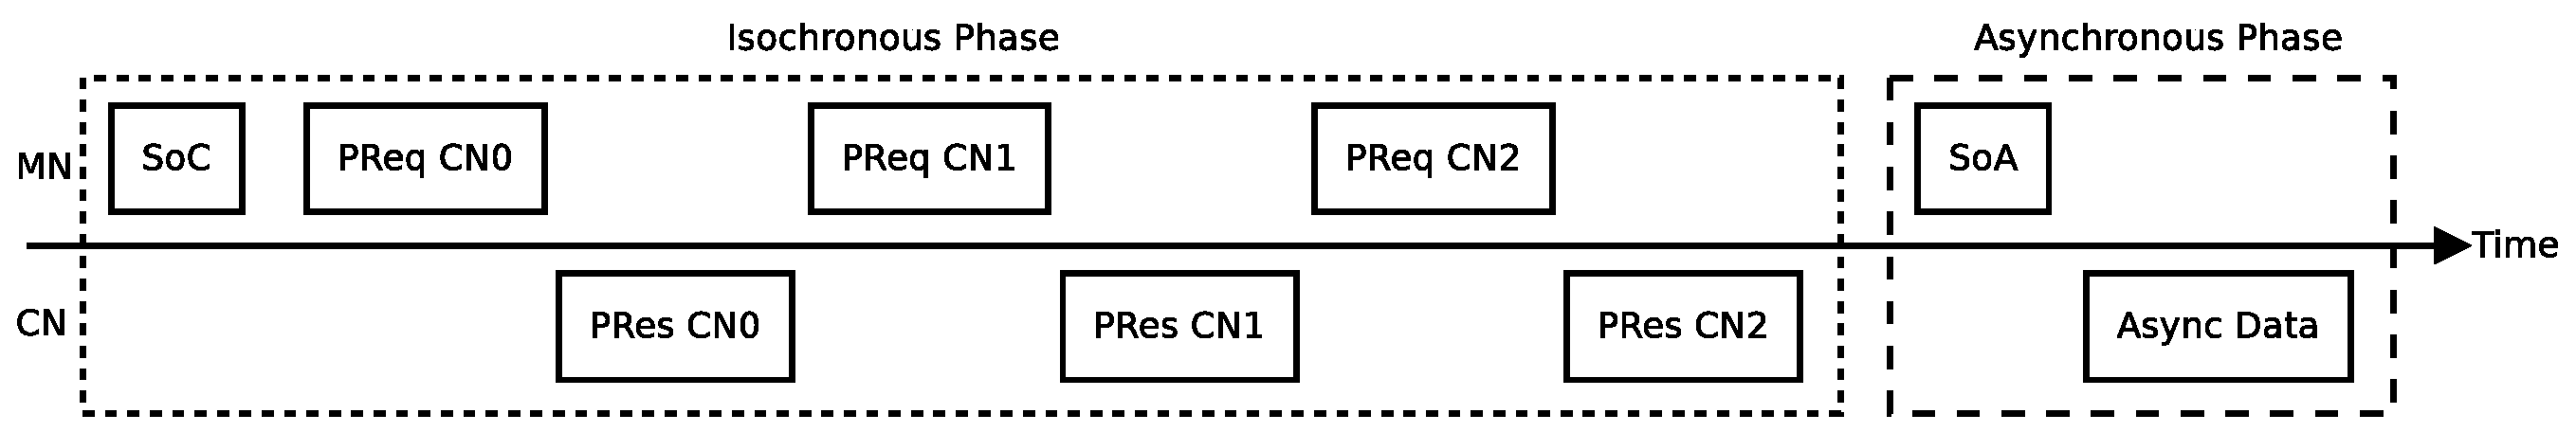
\includegraphics[width=0.95\linewidth]{powerlink_cycle}
    \caption{POWERLINK communication cylce containing Isochronous Phase with polling of three \emph{CNs} and Asynchronous Phase.}
    \label{fig:powerlink_cycle}
\end{figure}

The transmitted data within isochronous and asynchronous phase and the underlying object model are described in the following section.

\subsection{Data transmission}
\label{sec:oplk_powerlink_data_transmission}
The transmitted data objects are separated in two different groups.

The process data objects (\emph{PDO}) represent time critical data which is transmitted with each cycle.
This transmissions happens during the isochronous phase in the POWERLINK cycle and is enclosed in the \emph{Preq} and \emph{Pres} messages.

When the data of a \emph{PDO} is sent to other nodes it represents a transmit process data object (\emph{TPDO}).
Similar when the received data are stored in a \emph{PDO} this represents a receive process data object (\emph{RPDO}).

The implemented application defines the number of supported \emph{TPDOs} and \emph{RPDOs}, but those are limited to 256 for each type. \cite[section 6.4]{epsg_epsg_2013}
\\

The counterpart to the isochronous transmitted \emph{PDOs} are the service data objects \emph{SDOs}.
\emph{SDOs} provide access to an object within the \emph{OD} of any node within the POWERLINK network.
This access is follows the client-server principle, i.e. the \emph{SDO} client requests the value of an object located inside of the object dictionary (\emph{OD}) of the server.
After receiving the request, the \emph{SDO} server replies with the according data set.
The transmission of these data and the according commands are located within in the asynchronous phase of the POWERLINK cycle.
The granting of sending an asynchronous command is done by the \emph{MN}.

Different functions for accessing the \emph{OD} of the \emph{SDO} server are provided.
More information about the concrete functions for reading and writing a \emph{SDO} can be found in \cite[section 6.3.2.4.2]{epsg_epsg_2013};
\\

The mentioned \emph{OD} contains the definitions of all accessible objects within a POWERLINK network and is described in the next section.

\subsection{Object Dictionary}
\label{sec:oplk_powerlink_object_dictionary}
The \emph{OD} represents a collection of all defined objects which are transmitted via \emph{PDO} or \emph{SOD}, their types and additional communication objects.
Within the \emph{OD} every object is structured in the same way and can represent either a variable, an array or a record of multiple variables.
An object of type array or record contains multiple sub objects which must be of type variable.
Within the \emph{OD} different regions contains definitions for different types and various profiles. \cite[section 2.2.2]{epsg_epsg_2013}

Each object defined in the \emph{OD} consists of the following associated values.

\begin{description}
    \item[Index] represents an identifier of the object within the \emph{OD}.
    \item[Name] is the name of the object.
    \item[Object type] represents the type of the object (variable, array, record).
    \item[Data type] defines the type of the contained data.
    \item[Value range] defines an allowed value range for this object.
    \item[Access] defines the allowed access functions for this object.
    \item[PDO mapping] defines the available mapping possibilities to an \emph{PDO}.
    \item[Default value] defines the value of an uninitialized object.
    \item[Actual value] represents the current value of the object.
\end{description}

More information about the different associated values and further information to the definitions of the \emph{Access} and \emph{PDO mapping} field can be found in \cite{openpowerlink_od_object}.
\\

The openPOWERLINK stack implements the above described functionalities of POWERLINK.
Different demo applications, drivers and the stack implementations are contained in the openPOWERLINK stack distribution.
An introduction in the structure of the stack is given in the following section.


\section{Structure of the openPOWERLINK stack}
\label{sec:oplk_structure}
The openPOWERLINK stack distribution package is structured in different main directories containing demo applications, documentation, driver implementation, stack sources and many more.

For this paper the most important parts are the stack sources and demo applications.
Furthermore an additional simulation directory will be added whose content will be discussed in section \ref{sec:porting_simstub_sim}.

The \emph{apps} folder contains different demo application for embedded targets, linux and windows operating systems.
These demo applications contain exemplary implementations of \emph{MNs} and \emph{CNs}.
These application are analyzed for the development of demo applications within OMNeT++, as described in the section \ref{sec:porting_demo}.

The stack folder contains the following structure. \cite[Directory Structure]{openpowerlink_doc}
\begin{description}
    \item[build] represents the build directory for output files of the build process.
    \item[cmake] contains configuration files for the build tool chain.
    \item[include/oplk] represents the main include directories for all applications using the openPOWERLINK stack.
    \item[include/common] represents a common internal include directory.
    \item[include/kernel] represents an internal include directory for kernel modules.W
    \item[include/target] represents an internal include directory with target specific files.
    \item[include/user] represents an internal include directory for user modules.
    \item[lib] represents the installation directory for the openPOWERLINK libraries.
    \item[proj] represents the directory containing different library projects.
    \item[src/arch] represents a source directory with architecture specific functions.
    \item[src/common] represents a source directory with sources for user and kernel layer.
    \item[src/user] represents a source directory with sources for the user layer.
    \item[src/kernel] represents a source directory with sources for the kernel layer.
\end{description}

This structure represents the architecture of the openPOWERLINK stack, which is explained in the following section.

\section{Architecture}
\label{sec:oplk_architecture}

The openPOWERLINK stack is generally separated in kernel and user layer.
This separation was introduced with the version 2.X of the openPOWERLINK stack and is detaching the higher level user functionalities from the lower level kernel functions including time critical behavior and hardware drivers.
This separation of high level functionalities and time critical procedures allows a real-time communication independent of the running application and the executed user functions.

The separation of kernel and user layer using the communication abstraction layer (\emph{CAL}) is shown in figure \ref{fig:openpowerlink_arch}.

\begin{figure}
\centering
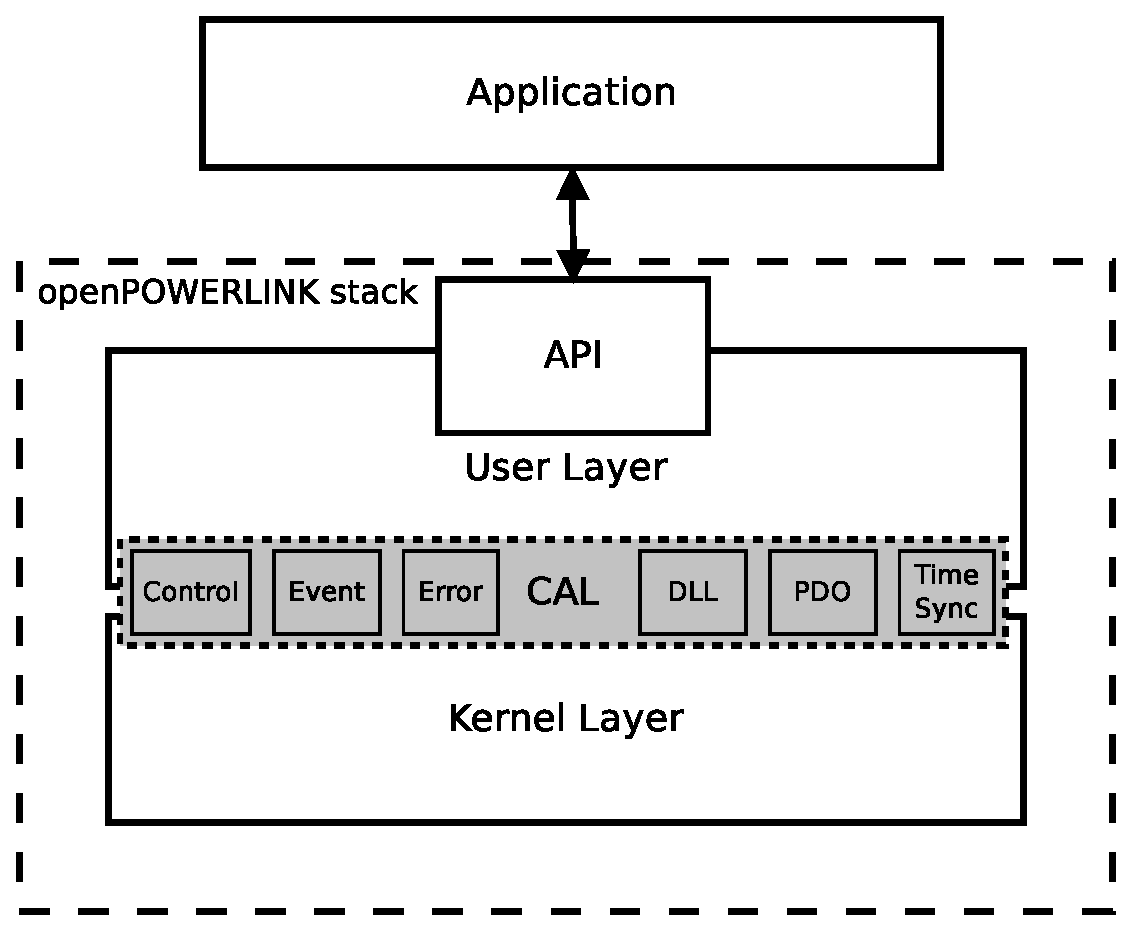
\includegraphics[width=0.9\linewidth]{images/openpowerlink_arch}
\caption{Software architecture of the openPOWERLINK stack.}
\label{fig:openpowerlink_arch}
\end{figure}


\subsection{Kernel layer}
\label{sec:oplk_architecture_kernel}

The kernel layer of the openPOWERLINK stack contains the following modules. \cite[openPOWERLINK Kernel Layer]{openpowerlink_doc}

\begin{description}
    \item[Control module] manages shutdown and startup commands for the kernel stack.
    \item[Data link layer (\emph{DLL}] implements the \emph{DLL} state machine and handles the creating and processing of the POWERLINK cycle.
    \item[Error handler] implements the POWERLINK error handler and manages the error counters.
    \item[Event handler] provides functionalities for posting events to other kernel modules and to the user layer.
    This handler also processes events posted by the user layer.
    \item[Led module] controls the POWERLINK status and error Leds.
    \item[\emph{PDO} module] handles the \emph{PDOs} in the openPOWERLINK kernel layer and communicates with the \emph{DLL} module for the transmission of the \emph{PDO}s.
    \item[Network management (\emph{NMT} module)] implements the \emph{NMT} state machine and provides the general functions for network management.
    \item[Virtual Ethernet driver] provides a network interface for sending Ethernet packets.
    These packets will be transmitted during the asynchronous phase.
    \item[High resolution timer module] provides high resolution timer functionalities for timing the POWERLINK cycle.
    \item[Synchronization timer module] implements the synchronization of a \emph{CN} to the POWERLINK cycle.
    \item[Timestamp module] provides helper functions for handling of timestamps.
    \item[Time synchronization module] implements the time synchronization to the POWERLINK network.
\end{description}

Running on an operating system, e.g. linux, the kernel layer can be built and executed separately as a kernel module of the operating system.
Such a communication mode is defined via the configurations of the different stack projects (proj folder).
The configurations are affecting the communication abstraction layer \emph{CAL} described in section \ref{sec:oplk_architecture_cal}.

\subsection{User layer}
\label{sec:oplk_architecture_user}

The user layer includes higher level functions and provides the application programming interface (\emph{API}) for an application using the openPOWERLINK stack.
The following modules are located within the user layer. \cite[openPOWERLINK User Layer]{openpowerlink_doc}

\begin{description}
    \item[API] represents the interface to the application and provides all functions for interactions with the openPOWERLINK stack.
    \item[Control module] manages shutdown and startup commands for the user stack.
    \item[Error handler] handles the synchronization of error counters located in the kernel layer with the according objects in the \emph{OD}.
    \item[Event handler] provides functionalities for posting events to other user modules and to the kernel layer.
    This handler also processes events posted by the kernel layer.
    \item[\emph{PDO} module] handles exchanging of process image data via the process image \emph{API}.
    \item[\emph{SDO} modules] provide the \emph{SDO} stack of openPOWERLINK including command layer, sequence layer and the transmission implementation using \emph{ASnd} or \emph{UDP}.
    \item[Network management (\emph{NMT} modules)] implements various \emph{NMT} functions of the user layer including functions for \emph{MN} and \emph{CN} and the handling of the \emph{Ident}-, \emph{Status}- and \emph{Sync}-requests.
    \item[Configuration manager module] implements the handling of the \emph{CDC} file and the configuration of connected \emph{CNs} using \emph{SDO} transmission.
    \item[\emph{OD} module] implements the POWERLINK \emph{OD}.
    \item[\emph{OD} abstraction layer] provides an abstraction layer for accessing different POWERLINK \emph{ODs}.
    \item[Timer module] implements timer functionalities used by the user stack modules.
    \item[Time synchronization module] provides a configurable notification at a specific synchronization point for the application.
\end{description}

\subsection{Communication abstraction Layer}
\label{sec:oplk_architecture_cal}

The user and kernel layer are separated by the communication abstraction layer (\emph{CAL}).
This layer is separated in different modules for each module within kernel and user layer which must communicate with the opposite module.
The separation of the \emph{CAL} and placement between the kernel and user layer is shown in figure \ref{fig:openpowerlink_arch}.
The gray dotted box shows the \emph{CAL} and all embedded modules using a \emph{CAL} related implementation.

The following modules use \emph{CAL} modules for communication between kernel and user layer. 

\begin{itemize}
    \item control module
    \item event handler
    \item error handler
    \item data link layer (\emph{DLL})
    \item process data objects (\emph{PDO})
    \item time sync
\end{itemize}

For the listed modules two \emph{CAL} modules are necessary within user and kernel layer.
Using a specific \emph{CAL} implementation must be configured in both layers.
Different implementations of the \emph{CAL} modules allow various configurations and compositions of the openPOWERLINK stack using different communication methods between kernel and user layer. \cite[CAL]{openpowerlink_doc}

\subsection{Hardware abstraction}
\label{sec:oplk_architecture_hardware}
The openPOWERLINK stack implements the support of different operating systems and hardware platforms by definition of the modules functions in a common header.
The compiled implementation represents the specification for each platform.

The platform dependency of the openPOWERLINK stack and the platform dependent modules are analyzed in section \ref{sec:oplk_platform}.

The dependency of the platform regarding byte endianess is handled by the abstract memory interface described in the next section.

\subsection{Abstract memory interface}
\label{sec:oplk_architecture_ami}

The abstract memory interface (\emph{AMI}) provides multiple simple functions for the correct handling of data fields affected by the byte endianess.
Similar to the \emph{CAL} and hardware abstraction the implementations for different platforms are defined by compiling the according implementation. \cite[AMI]{openpowerlink_doc}
\\

The openPOWERLINK stack provides multiple configurable implementation and communication variants.
These are manages within the used tool chain described in the next section.

\section{Configuration and build}
\label{sec:oplk_build}
For configuration and building of the openPOWERLINK stack the built tool \emph{CMAKE} is used.
The main \emph{CMAKE} file \emph{CMakeLists.txt} checks the current \emph{CMAKE\_SYSTEM\_NAME} variable and uses the according configuration matching the targeted platform.

The global \emph{CMAKE} file loads according to the \emph{CMAKE\_SYSTEM\_NAME} and \emph{CMAKE\_SYSTEM\_PROCESSOR} variable the correct system specific options file.
This option file includes options for enabling and disabling part of the openPOWERLINK stack.
For example the generation of the \emph{CN} or \emph{MN} library can be en- or disabled.
Further options are platform specific and provide configuration possibilities for various features available in different implementations and on different platforms.

Requires the targeted platform a custom tool chain so a specific tool chain file must be defined containing configurations regarding the used tool chain.

The \emph{CAL}, hardware abstraction and \emph{AMI} are using specific implementations of common header files.
These sets of specific sources are defined within the common \emph{CMAKE} file \emph{stackfiles.cmake}.
This file includes groups defined source files for each module and each implementation specialization.
The usage of such specific groups is done in project specific \emph{CMAKE} files composing various stack variants for specific platforms. \cite[Building openPOWERLINK]{openpowerlink_doc}

Within the system specific options file all defined projects matching this system are included in the configuration.
These projects are located in the \emph{proj} folder as described in the following section.

\subsection{Library projects}
\label{sec:oplk_structure_proj}
Located in the \emph{proj} folder various projects for different systems are defined.
These projects are grouped in the following systems.

\begin{description}
    \item[generic] contains projects for embedded targets without underlying operating systems.
    \item[linux] contains projects for linux operating systems.
    \item[windows] contains projects for windows operating systems.
\end{description}

Within each system specific folder different projects are located.
These different projects use different features and functionalities of the openPOWERLINK stack.
Within the different project directories the \emph{CMakeLists.txt} file defines the used implementations and sources.
The groups defined in the \emph{stackfiles.cmake} file are used and combined within the project specific \emph{CMAKE} file.

Additional configurations made by preprocessor defines are set in the \emph{oplkcfg.h} header file within each project directory.
\\

Executing the \emph{CMAKE} build tool generates the according makefile.
Using this makefile either all included or specific projects can be built and installed at a defined install directory. \cite[Building Stack Libraries]{openpowerlink_doc}

\section{Platform dependency}
\label{sec:oplk_platform}

The openPOWERLINK uses specific implementations implementing a common header file for supporting multiple platforms.
As described in the sections \ref{sec:oplk_architecture_cal}, \ref{sec:oplk_architecture_hardware} and \ref{sec:oplk_architecture_ami} this strategy is used for the \emph{CAL}, hardware dependencies and \emph{AMI}.

These three categories of modules represent the platform dependency of the openPOWERLINK stack.
The informations about these modules and their features are taken from the naming convention of platform specific implementations, i.e. an appended suffix with the abbreviation for the specific implementation type.
The following sections will refer to those suffixes as the implementation types.
Detailed information about the functionality of each module can be found at the header comment of each implementation file describing the designated usage and the used functions.

In the following sections each one of the modules and their specific implementations are analyzed and the platform dependent functionalities are shown.

\subsection{CAL}
\label{sec:oplk_platform_cal}

The \emph{CAL} includes multiple modules providing configurable implementations using different platform specific functionalities.
The following listings show the different available implementations of the \emph{CAL} modules, which is followed by the description of the different implementations and their included functionalities.
\\
    
\begin{description}[leftmargin=0cm]
    \item[control module] \mbox{}
    \begin{multicols}{3}
        \begin{itemize}
            \item direct
            \item hostif
            \item mem
            \item noosdual
            \item pcie
            \item ioctl
            \item winioctl
        \end{itemize}
    \end{multicols}
    
    \item[event handler] \mbox{}
    \begin{multicols}{3}
        \begin{itemize}
            \item linux
            \item linuxkernel
            \item linuxioctl
            \item linuxpcie
            \item nooscircbuf
            \item noosdual
            \item nooshostif
            \item win32
            \item winkernel
            \item winioctl
            \item winpcie
        \end{itemize}
    \end{multicols}
    
    \item[error handler] \mbox{}
    \begin{multicols}{3}
        \begin{itemize}
            \item hostif
            \item ioctl
            \item local
            \item noosdual
            \item posixshm
            \item winioctl
        \end{itemize}
    \end{multicols}
    
    \item[DLL] \mbox{}
    \begin{multicols}{3}
        \begin{itemize}
            \item circbuff
            \item ioctl
            \item winioctl
        \end{itemize}
    \end{multicols}
    
    \item[PDO] \mbox{}
    \begin{multicols}{3}
        \begin{itemize}
            \item triplebufshm
            \item hostif
            \item linuxkernel
            \item local
            \item noosdual
            \item posixshm
            \item winkernel
            \item linuxmmap
            \item linuxpcie
        \end{itemize}
    \end{multicols}
    
    \item[time sync] \mbox{}
    \begin{multicols}{3}
        \begin{itemize}
            \item bsdsem
            \item hostif
            \item ioctl
            \item local
            \item noosdual
            \item winioctl
            \item linuxkernel
            \item winkernel
        \end{itemize}
    \end{multicols}
\end{description}

The different implementations using specific functionalities are often used for multiple modules.
The used functionalities of the different implementations are described in the following listing defined by the postfix of the implemented modules.

\begin{description}
    \item[direct] This implementations use direct calls between kernel and user layer.
    This is supported in configurations when both layers are located in the same instance.
    \item[hostif/nooshostif] This implementations use the host interface ip core instantiated on an FPGA.
    \item[noosdual] This implementations target platforms without operating system but providing a dual processor and a shared memory between them.
    This shared memory is used for various communications.
    \item[nooscircbuf] This implementations use the circularbuffer library targeting platforms without underlying operating system.
    \item[linux] This implementations use the circularbuffer library with both layer located in the Linux user space.
    \item[linuxkernel] This implementations represent the interface of the Linux kernel space module which includes the kernel layer and can be accessed via ioctl.
    \item[ioctl/linuxioctl] This implementations represent the counterpart for \emph{linuxkernel} and communicate with the kernel module via ioctl.
    \item[pcie/linuxpcie] This implementations use ioctl for communication with the Linux PCIe driver and furthermore communicating with an external device connected via PCIe and running the kernel layer.
    \item[linuxmmap] This implementations provide a memory interface with a memory mapping between kernel and user layer separated in user application and kernel module.
    \item[win32] This implementations use the circularbuffer library with both layer located in the Windows user space.
    \item[winkernel] This implementations represent the interface of the Windows kernel space module which includes the kernel layer and can be accessed via ioctl.
    \item[winioctl] This implementations represent the counterpart for \emph{winkernel} and communicate with the kernel module via ioctl.
    \item[winpcie] This implementations use ioctl for communication with the Windows PCIe driver and furthermore communicating with an external device connected via PCIe and running the kernel layer.
    \item[local] This implementations use global variables for data storage and requires kernel and user layer running in the same domain for sharing global variables.
    \item[posixshm] This implementations use posix shared memory for communication between kernel and use layer.
    \item[triplebufshm] This implementations use a triple buffer implementation for synchronous reading and writing of a shared memory.
    The shared memory can be configured due to the usage of a abstraction given by a common header file.
    \item[bsdsem] This implementations use BSD semaphores for synchronization of kernel and user layer.
\end{description}



\subsection{Hardware abstraction}
\label{sec:oplk_platform_hardware}

As described in section \ref{sec:oplk_architecture_hardware} the hardware abstraction is done in a similar way as the \emph{CAL} by using specific implementations of common header files.
The following listing includes all hardware dependent modules, their location within the stack directories, a summary of the provided functionalities and their available implementation types.

\begin{description}[leftmargin=1cm]
    \item[target] The \emph{target} module is located in the \emph{arch} folder and provides target specific functions controlling the defined IP address, default gateway, global interrupt, status/error leds and a sleep function.
    This module is separated in different folder containing implementations for the following specific platforms and systems.
    \begin{multicols}{3}
        \begin{itemize}
            \item altera-c5socarm
            \item altera-nio2
            \item linux
            \item linuxkernel
            \item windows
            \item winkernel
            \item xilinx-microblaze
            \item xilinx-zynqarm
        \end{itemize}
    \end{multicols}
    These folders can also include different implementations for specific functions.
    The different types are similar to the listed specific implementations of the \emph{CAL} shown in \ref{sec:oplk_platform_cal}.\\
    
    \item[circularbuffer] The \emph{circularbuffer} module is located in the \emph{common} folder and provides an implementation for reading and writing variable sized data segments from and to a circular buffer.
    This module contains different implementations regarding the location of the used memory and the handling of memory access.
    These different implementations use system specific functionalities for locking and synchronizing memory access.
    Those implementations are used by the generic \emph{circularbuffer} implementation using the \emph{circbuf-arch} interface.
    The different implementation types of this interface are shown in the following listing.
    \begin{multicols}{3}
        \begin{itemize}
            \item linuxkernel
            \item noos
            \item noosdual
            \item nooshostif
            \item posixshm
            \item win32
            \item winkernel
        \end{itemize}
    \end{multicols}
    The used functionalities are similar to the described specific implementations of the \emph{CAL} shown in \ref{sec:oplk_platform_cal}.\\
    
    \item[memmap] The \emph{memmap} module is located in the \emph{common} folder and provides implementations for the handling of memory mapping used in various modules, e.g. \emph{CAL} modules.
    This module contains different implementations regarding the location of the used memory and the handling of memory access.
    These implementations use different functionalities providing a common interface for memory mapping.
    The available implementation types are shown in the following listing.
    \begin{multicols}{3}
        \begin{itemize}
            \item linuxpcie
            \item noosdual
            \item nooshostif
            \item nooslocal
            \item null
            \item winioctl
        \end{itemize}
    \end{multicols}
    The used functionalities are similar to the described specific implementations of the \emph{CAL} shown in \ref{sec:oplk_platform_cal}.\\
    
    \item[edrv] The \emph{edrv} module is located in the \emph{kernel} folder and provides implementations of various Ethernet drivers.
    This driver provides functionalities for Ethernet communication and settings regarding the underlying Ethernet controller.
    The following implementation types of Ethernet drivers supporting different types of Ethernet controller are available.
    \begin{multicols}{3}
        \begin{itemize}
            \item Realtek 8111
            \item Realtek 8139
            \item Intel 8255x
            \item Intel 82573
            \item emacps
            \item Intel i210
            \item mux\_vxworks
            \item ndisintermediate
            \item openmac
            \item pcap\_linux
            \item pcap\_win
        \end{itemize}
    \end{multicols}
    The implemented versions for the different Ethernet controller are implemented for the custom behavior and usage of different controllers and libraries.
    \\
    
    \item[hrestimer] The \emph{hrestimer} module is located in the \emph{kernel} folder and provides implementations for various high resolution timer drivers.
    These timers are necessary for timing the POWERLINK cycle and for the synchronizing to the POWERLINK network.
    Depending on the implementation either a connection to a hardware or software component providing the required resolution is used.
    The following list shows the different supported high resolution timers.
    \begin{multicols}{3}
        \begin{itemize}
            \item Intel i120
            \item linuxkernel
            \item ndistimer
            \item openmac
            \item posix
            \item posix-clocknanosleep
            \item vxworks
            \item windows
            \item zynqttc
        \end{itemize}
    \end{multicols}
    Those different implementations use different components as timers.
    
    \item[veth] The \emph{veth} module is located in the \emph{kernel} folder and provides implementations of different virtual Ethernet driver.
    This driver provides the functionality of receiving a non POWERLINK Ethernet frame and passing this to the user layer.
    The different implementations use different functionalities of underlying systems and platforms for synchronization and communication.
    The available implementations are shown in the following list.
    \begin{multicols}{3}
        \begin{itemize}
            \item generic
            \item linuxkernel
            \item linuxpcie
            \item linuxuser
            \item ndisintermediate
        \end{itemize}
    \end{multicols}
    The used functionalities are similar to the described specific implementations of the \emph{CAL} shown in \ref{sec:oplk_platform_cal}.\\
    
    \item[sdo] The \emph{sdo} module is located in the \emph{user} folder and provides implementations for transmitting the \emph{SDOs} during the asynchronous phase.
    This transmission can be done via a \emph{ASnd} message or an legacy Ethernet frame, as described in section \ref{sec:oplk_powerlink_data_transmission}.
    Performing this transmission by using legacy Ethernet frames the User Datagram Protocol (\emph{UDP}) is used for data transmission based on the Internet Protocol (\emph{IP}).
    The implementation of the \emph{UDP} and \emph{IP} creation can be done in various ways due to the available \emph{UDP} and \emph{IP} stacks on operating systems.
    Therefore this module provides different implementations for different platforms providing the usage of Linux and Windows functionalities.
    Additionally the open library \emph{socketwrapper} can be configured which allows the integration of an custom \emph{UDP} stack.
    The following list shows the available implementations
    \begin{multicols}{3}
        \begin{itemize}
            \item linux
            \item windows
            \item socketwrapper
        \end{itemize}
    \end{multicols}
    The implementations for Linux and Windows are using the existing functionalities for creation and handling of \emph{UDP} sockets.\\
    
    
    \item[timer] The \emph{timer} module is located in the \emph{user} folder and provides different implementations for timer functionalities used by the user layer.
    These timer functions does not require the high resolution and accuracy of the \emph{hrestimer} module and can therefore be implemented simpler and use less resources.
    The different implementations include a generic implementation using the global system tick and specific implementations using features of underlying operating systems.
    These types of implementations are shown in the following list.
    \begin{multicols}{3}
        \begin{itemize}
            \item generic
            \item linuxkernel
            \item linuxuser
            \item vxworks
        \end{itemize}
    \end{multicols}
    Does the target system not provide such a functionality or the requirement for a high precision user timer is not given the usage of the generic implementation is sufficient.\\
        
        
\end{description}

\subsection{AMI}
\label{sec:oplk_platform_ami}

The \emph{AMI} (described in section \ref{sec:oplk_architecture_ami}) represents also a platform dependent module and therefore provides different implementations for little- and big-endian processors.
Additionally an optimized implementation for x86 processors is provided.

None of these implementations use platform specific functionalities, but the implementation varies for achieving the correct result when handling with variable consisting of multiple bytes.
\\

The platform dependencies of the openPOWERLINK stack shown in this section represents those modules which must be customized for porting the openPOWERLINK stack to a new platform or in a new environment.
The porting of the openPOWERLINK stack in an simulation environment using OMNeT++ and the development of the according simulation is shown in the following chapter.